Without loss of generality, let us focus on one particular source of uncertainty: the subthreshold leakage current and, more specifically, on the effective channel length. The reason for this choice is that the effective channel length has the strongest influence on leakage \cite{juan2011, juan2012}; in particular, it also affects the threshold voltage. Consequently, in what follows, $\u$ stands for this major parameter, the channel length.

\begin{figure}
  \centering
  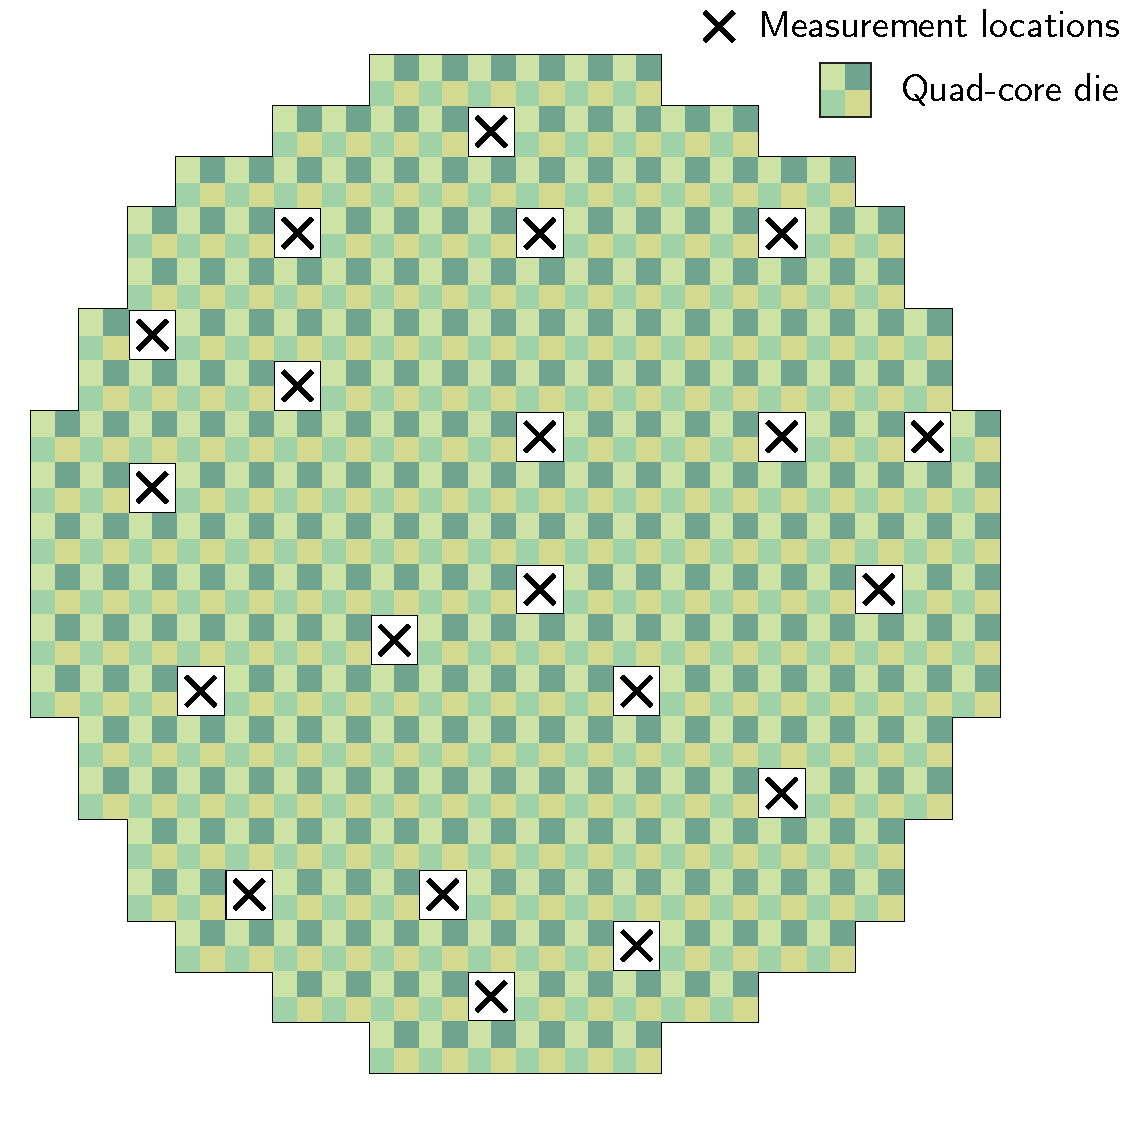
\includegraphics[width=0.7\linewidth]{include/assets/wafer-pick.pdf}
  \caption{A wafer with 316 quad-core dies.}
  \flabel{wafer-pick}
  \vspace{-1.5em}
\end{figure}

\begin{figure}
  \centering
  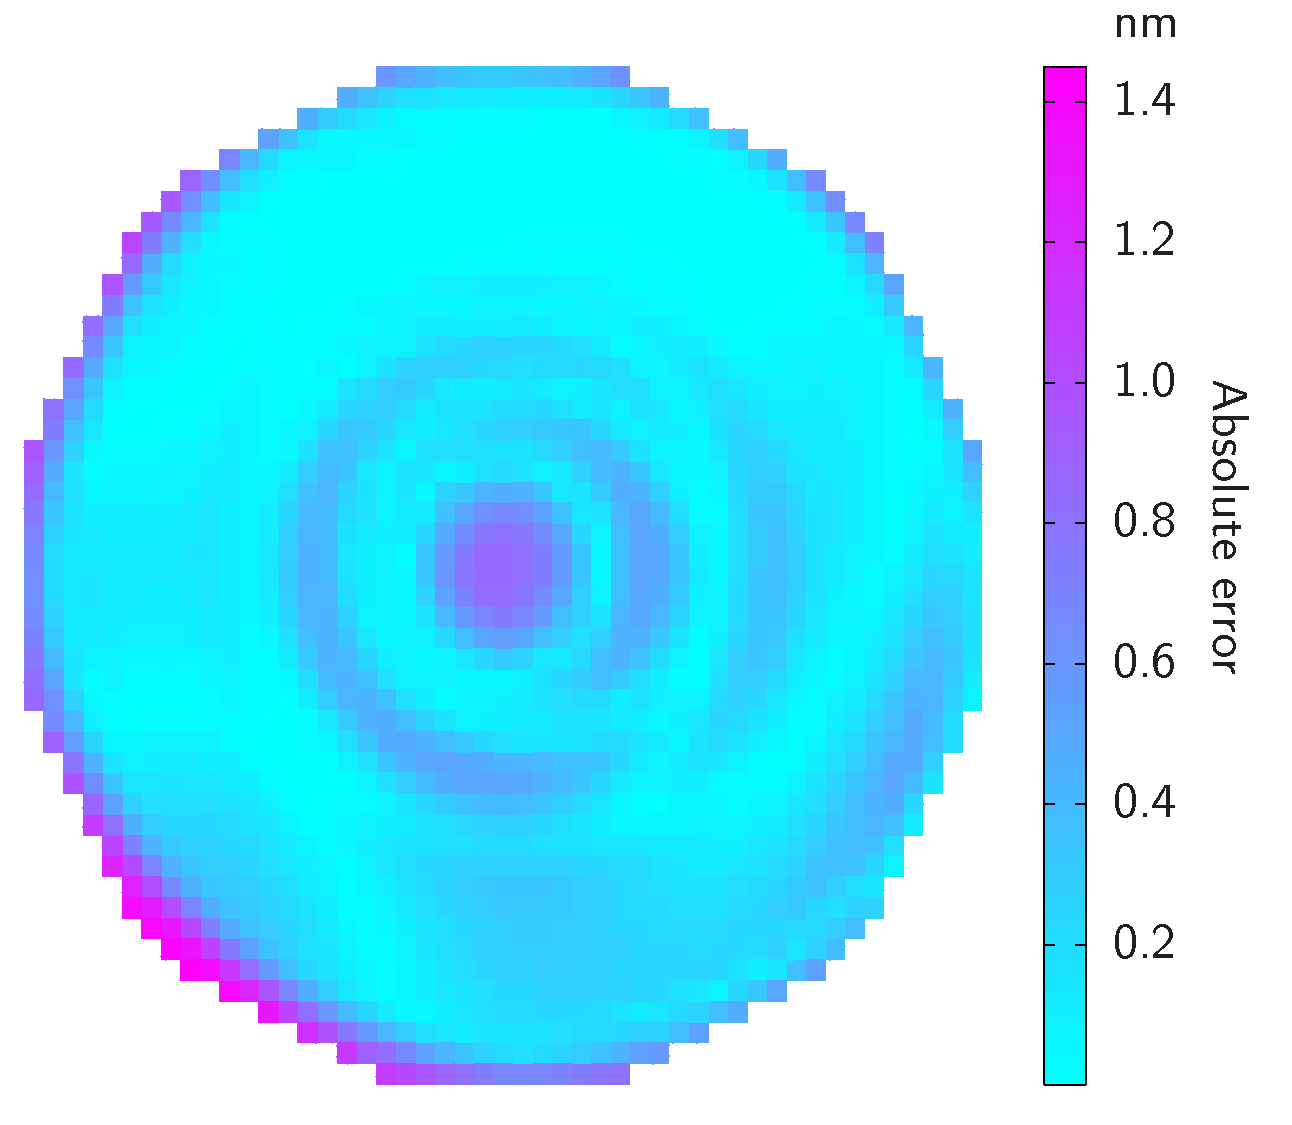
\includegraphics[width=0.6\linewidth]{include/figures/wafer-qoi-error.pdf}
  \caption{Absolute error across the wafer.}
  \flabel{wafer-qoi-error}
\end{figure}

Now, we shall describe the default configuration of our experimental setup, which, in the following subsections, will be adjusted according to the purpose of a particular experiment. We consider a 45-nanometer technological process. The wafer is assumed to be inscribed in a square with $20 \times 20$ even cells. The total number of dies $\nchips$ is 316, and the number of processing elements $\nprocs$ on each of the dies is four. The number of spacial measurements $\ndata$ is 20. These locations (dies) are chosen as follows: the first one is place in the middle of the wafer, and the rest are selected sequentially such that the total distance from the already picked dies and the new one to the left dies is minimized. In this way, we pursue uniformity of the wafer coverage. An example is depicted in \fref{wafer-pick}. The floorplans of the multiprocessor platforms are constructed in such a way that the processing elements form regular grids, as it is the case with, \eg, Alpha 21264 studied in \cite{juan2011}. The capacitance and conductance matrices in \eref{heat-de} are obtain using HotSpot v5.02 \cite{hotspot}. The dynamic power profiles involved in the experiments are based on simulations of randomly generated task graphs using TGFF v3.5 \cite{dick1998}.\footnote{The floorplans of the platforms, thermal configuration of HotSpot, task graphs of the applications, etc. are available online at \cite{sources}.} The sampling interval of these profiles is $1~\text{ms}$. The number of temporal measurements $\nsteps$ is 20. These time moments are chosen to be evenly spaced and to cover the whole time spans of the corresponding dynamic power profiles  $\profilePdyn$ (the total number of steps $\npsteps$ is typically much larger).

Let us turn to the statistical model in \sref{statistical-model}. In the covariance function given by \eref{covariance-function}, the weight parameter $\eta$ is 0.7 prioritizing the squared exponential kernel, and both length-scale parameters, $\ell_\SE$ and $\ell_\OU$, are set to half the radius of the wafer. The threshold parameter in the model order reduction procedure described in \sref{kl-expansion} is set to $0.99$ preserving $99\%$ of the variance of the data; the number of the resulting \rvs, \ie, the dimensionality of $\vz$ in \eref{kl-approximation}, $\nvars$, was found to be around 27. In the prior for the mean of $\u$ (see \eref{mu-u-prior}), we let $\mu_0$ be $45~\text{nm}$ and $\sigma_0$ be $1\%$ of $\mu_0$. The later represents our rather high certainty about the expected value of $\u$ as it is a part of the specification of the technological process. In the prior for the variance of $\u$ (see \eref{sigma2-u-prior}), we let $\tau_\u$ be $5\%$ of the mean value \cite{juan2011, juan2012}, and $\nu_\u$ is set to ten. The later has an intuitive interpretation in the Bayesian context: $\nu_\u$ can be thought of as being the number of imaginary observations (prior to actual observations) that the decision about $\tau_\u$ is based on. In the prior for the variance of noise (see \eref{sigma2-noise-prior}), we let $\tau_\noise$ be $1~\text{K}$ (Kelvin), and $\nu_\noise$ be ten observations (the same meaning as for $\nu_\u$). To summarize the reasoning behind the priors, the hyperparameters $\mu_0$, $\tau_\u$, and $\tau_\u$ represent the presumable values of $\mu_u$, $\sigma_\u$, and $\sigma_\noise$, respectively, and the hyperparameters $\sigma_0$, $\nu_\u$, and $\nu_\noise$ reflect the degree of our beliefs according to our prior knowledge. In the absence of such knowledge, non-informative priors can be chosen; refer to \cite{gelman2004} for further details. The tuning constant $\alpha$ in \eref{proposal} is set to 0.5. The optimization procedure (recall \sref{proposal-distribution}) is limited by $10^4$ objective function evaluations (the log-posterior in \eref{log-posterior}). The number of samples that we draw from the posterior is $10^4$; the first half of these samples is discarded leaving $5 \cdot 10^3$ effective samples $\nsamples$. Unless otherwise stated, the number of processes performing the Metropolis sampling in parallel is four.\footnote{All the experiments have been conducted on a GNU/Linux machine with Intel Core i7 2.66~GHz and 8~GB of RAM.}

\subsection{In-depth Analysis}
\begin{figure}
  \centering
  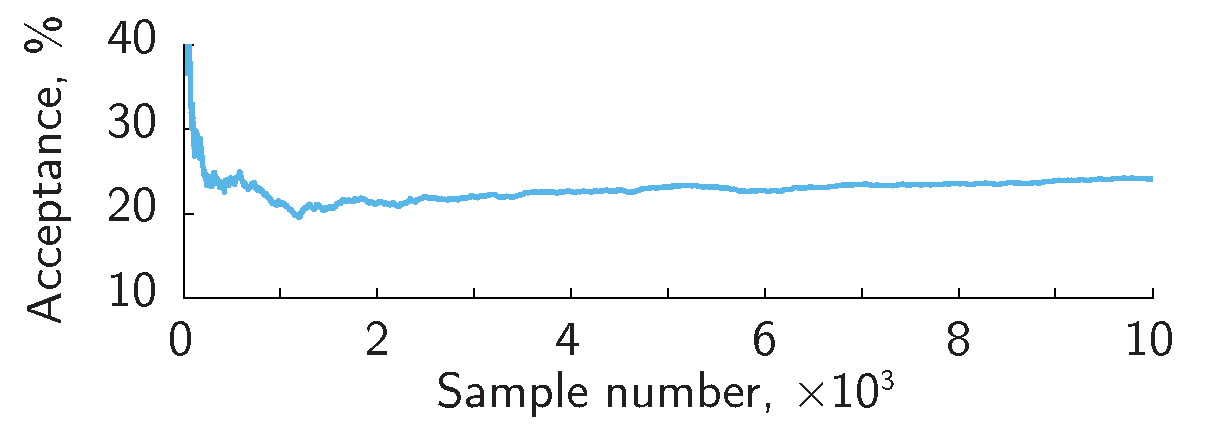
\includegraphics[width=0.7\linewidth]{include/figures/acceptance.pdf}
  \caption{Evolution of the acceptance rate.}
  \flabel{acceptance}
  \vspace{-0.5em}
\end{figure}

\begin{figure}
  \centering
  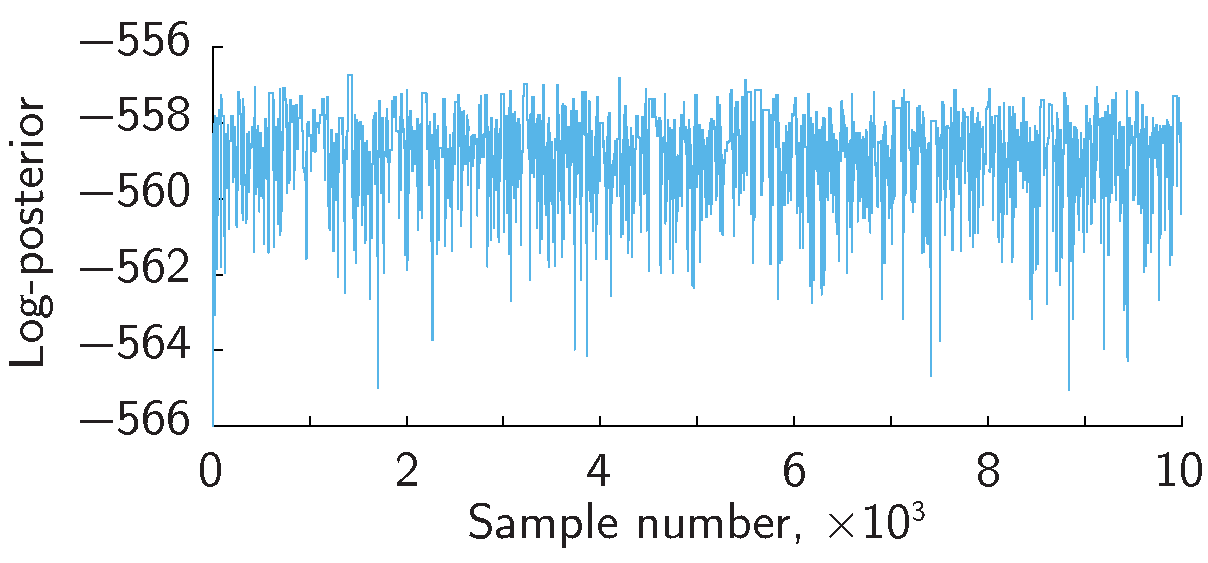
\includegraphics[width=0.7\linewidth]{include/assets/log-posterior.pdf}
  \caption{Evolution of the log-posterior.}
  \flabel{log-posterior}
  \vspace{-1.5em}
\end{figure}

\begin{figure}
  \centering
  \vspace{-1.5em}
  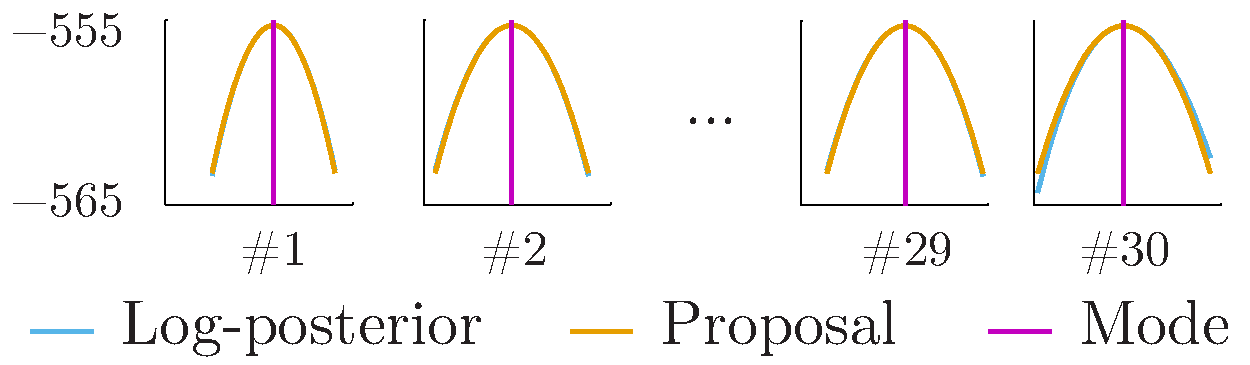
\includegraphics[width=0.8\linewidth]{include/figures/proposal.pdf}
  \caption{Inspection of the proposal.}
  \flabel{proposal}
\end{figure}

Let us first perform a detailed analysis of the results obtained for one particular example with the default configuration described earlier. The true and inferred distributions of the QoI are shown in \fref{wafer-qoi}. In this case, the normalized root-mean-square error (NRMSE) is below $2.8\%$, and the distribution across the wafer of the absolute error can be observed in \fref{wafer-qoi-error}. It can be seen that the framework produces a close match to the true value of the QoI. The graph in \fref{acceptance} displays the acceptance rate of the Metropolis algorithm, from which we conclude that algorithm, accepting $20$--$30\%$ of samples on average, agrees with the recommendations from the literature \cite{gelman2004}. We can also conclude that the constructed Markov chain vividly explores the probability space by looking at the log-posterior (up to a constant summand) in \fref{log-posterior}. One more test, common in statistics, to assess the quality of the proposal distribution is given in \fref{proposal}. Here, the proposal in \eref{proposal} is plotted along with the log-posterior in \eref{log-posterior} around the posterior mode $\hat{\vparam}$. Since, in this example, the dimension of $\vparam$ is 30, the number of such plots is also 30. The curves are nearly indistinguishable implying a high quality of the proposal. The above premises lead to the conclusion that the optimization and sampling procedures are fine-tuned.

\subsection{Number of Processing Elements}
In this subsection, we consider five platforms with the number of processing elements $\nprocs$ equal to 2, 4, 8, 16, and 32 cores, respectively. The results are summarized in \tref{processing-elements}.
\begin{table}[h]
  \centering
  \caption{Results for the number of processors $\nprocs$.}
  \begin{tabular*}{0.90\linewidth}{lrrrrr}
    \toprule
    Processing elements & 2 & 4 & 8 & 16 & 32 \\
    \midrule
    Time in sequence, m & 0 & 0 & 0 & 0 & 0 \\
    Time in parallel, m & 1.87 & 2.71 & 5.36 & 10.09 & 26.32 \\
    NRMSE, \%           & 4.50 & 3.62 & 3.92 &  2.69 &  1.82 \\
    \bottomrule
  \end{tabular*}
  \tlabel{processing-elements}
  \vspace{-1em}
\end{table}


\subsection{Number of Space Measurements}
In this subsection, we change the number of dies $\ndata$ for which the measurement data are available in the input data set $\Data$ (correspondingly, $\nchips - \ndata$ dies on the wafer are left unobserved). The considered scenarios are 1, 10, 20, 40, 80, and 160 dies.

\subsection{Number of Time Measurements}
In this subsection, we sweep the number of moments of time $\nsteps$ for which the measurement data are available in the input data set $\Data$ (correspondingly, $\npsteps - \nsteps$ steps are discarded after $\model$ is evaluated for the input power profile $\profilePdyn$). The considered scenarios are 1, 10, 20, 40, 80, and 160 moments of time.

\subsection{Measurement Noise}
In this subsection, we vary the level of the noise in the input data set $\Data$ within the set $\{ 0, 0.5, 1, 2 \}$ (in Kelvins) while keeping the corresponding prior distribution in \eref{sigma2-noise-prior} unchanged.

\subsection{Numerical vs. Analytical Solution}
In this subsection, we demonstrate the speedup due to the analytical solution of the forward model comparing with a numerical solution (see \sref{analytical-solution}).

\subsection{Na\"{i}ve vs. Optimized Proposal Distribution}
In this subsection, we show the importance of the optimization procedure preceding the sampling part (see \sref{proposal-distribution}).

\subsection{Sequential vs. Parallel Sampling}
In this subsection, we illustrate the difference between the two sampling strategies: sequential and parallel (see \sref{sampling-strategy}). Since the limit on the number of objective function evaluations of the optimization procedure and the number of sample draws (including the burn-in prior) is the same, \ie, equal to $10^4$, the two would take the same time to finish if the optimization reached the limit. In our experiments, however, this limit was never observed to be reached. Therefore, using the default setup without parallelization, the optimization always takes less time than sampling. The situation changes when parallel computing (with four workers, in our case) is plugged in: the sampling part decreases by approximately 2–3 times, which indicates good parallelization properties of the chosen sampling strategy.
